% LaTeX set-up adapted from a template by Alan T. Sherman (9/9/98)
%%%%%%%%%%%%%%%%%%%%%%%%%%%%%%%%%%%%%%%%%%%%%%%%%%%%%%%%%%%%%%%%%%%%%%
\documentclass[12pt]{article}
\usepackage[a4paper,bindingoffset=0.2in,left=0.75in,right=0.75in,top=1in,bottom=1in,footskip=.25in]{geometry}
\usepackage{amsmath}
\usepackage{amsfonts}
\usepackage{tabularx}
\usepackage{float}
\usepackage{color}
\usepackage{multicol}
\usepackage{graphicx}
\usepackage{subfig}
\DeclareGraphicsExtensions{.jpg}
\graphicspath{ {/home/anton/documents/masc/ml/matlab/strategy_naive/} }
\usepackage{algorithm}
\usepackage{algpseudocode}

% Set multicol stuff
\setlength{\columnseprule}{1pt}
\def\columnseprulecolor{\color{blue}}

% Set table floating
% use \begin{table}[H] to fix its position.
\restylefloat{table}

%%%%%%%%%%%%%%%%%%%%%%%%%%%%%%%%%%%%%%%%%%%%%%%%%%%%%%%%%%%%%%%%%%%%%%%
% Macros

% Math Macros.  It would be better to use the AMS LaTeX package,
% including the Bbb fonts, but I'm showing how to get by with the most
% primitive version of LaTeX.  I follow the naming convention to begin
% user-defined macro and variable names with the prefix "my" to make it
% easier to distiguish user-defined macros from LaTeX commands.
%
\newcommand{\myfunction}[3] {${#1} : {#2} \rightarrow {#3}$ }
\newcommand{\myzrfunction}[1] {\myfunction{#1}{{\myZ}}{{\myR}}}
\renewcommand{\iff}{\Leftrightarrow}
\newcommand{\pluseq}{\mathrel{+}=}
\newcommand{\mineq}{\mathrel{-}=}


% Formating Macros %

% header
\newcommand{\myheader}[4] {\vspace*{-0.5in} \noindent{#1} \hfill {#2} \newline \noindent{#3} \hfill {#4} \noindent \rule[8pt]{\textwidth}{1pt} \vspace{1ex} }
\newcommand{\myalgsheader}[0] {\myheader{MASc Research Weekly Update}{UTIAS SRG}{Anton Rubisov}{\today}} 
% end header

\newcommand\undermat[2]{% http://tex.stackexchange.com/a/102468/5764
  \makebox[0pt][l]{$\smash{\underbrace{\phantom{%
    \begin{smallmatrix}#2\end{smallmatrix}}}_{\text{$#1$}}}$}#2}
    
\newcommand\overmat[2]{%
  \makebox[0pt][l]{$\smash{\overbrace{\phantom{%
    \begin{smallmatrix}#2\end{smallmatrix}}}^{\text{$#1$}}}$}#2}
    
    
\newcommand\mat[1]{\boldsymbol{#1}}


%%%%%% Begin document with header and title %%%%%%%%%%%%%%%%%%%%%%%%%

\begin{document}
\myalgsheader
\pagestyle{plain}
{\begin{center} {\large {\bf Limit Order Book Dynamics}} \end{center}}
\bigskip

%%%%% Begin body %%%%%%%%%%%%%%%%%%%%%%%%%%%%%%%%%%%%%%%%%%%%%%%%%%%

\begin{quote}
Our goal is to use the dynamics of the Limit Order Book (LOB) as an indicator for
high-frequency stock price movement, thus enabling statistical arbitrage. Formally, we will the study limit order book imbalance process, $I(t)$, and the stock price process, $S(t)$, and attempt to establish a stochastic relationship $\dot{S} = f(S,I,t)$. We will then attempt to derive an optimal trading strategy based on the observed relationship.
\end{quote}

\section*{Recap Next Steps}
\begin{enumerate}
\item Complete in-sample backtesting of the `naive' trading strategies.
\item Formulate stochastic control problem 
\item Extra Reading: Bellman Equations, MDP, Partially Observable MDP
\end{enumerate}

\section*{In-Sample Backtesting of Naive Trading Strategies}
As a refresher: 

We are a considering a CTMC for the joint distribution $(I(t), \Delta S(t))$ where $I(t) \in \lbrace 1,2,\dots,\#_{bins} \rbrace$ is the bin corresponding to imbalance averaged over the interval $[t-\Delta t_I, t]$, and $\Delta S(t) = \text{sign}(S(t+\Delta t_S)-S(t)) \in \lbrace -1, 0, 1 \rbrace$, considered individually for the best bid and best ask prices. The pair $(I(t), \Delta S(t))$ was then reduced into one dimension with a simple encoding.

From the resulting timeseries we estimated a generator matrix $\mat{G}$ and used it to obtain a one-step transition probability matrix $\mat{P} = e^{\mat{G}\Delta t_I}$. The entries of $\mat{P}$ contain the conditional probabilities $\mathbb{P}\left[ \rho_{curr}, \Delta S_{curr} \; | \; \rho_{prev}, \Delta S_{prev} \right]$, from which we can solve for the probability of now seeing a given price change ($\Delta S_{curr}$) conditional on the current imbalance, the previous imbalance, and the previous price change.

For example, one such conditional probability matrix $\mat{P_C}$ (using 3 imbalance bins) was:

$$  \begin{smallmatrix}
    \Delta S_n < 0 \rightarrow \\
    \Delta S_n = 0 \rightarrow \\
    \Delta S_n > 0 \rightarrow
  \end{smallmatrix}
  \left [
    \begin{smallmatrix}
\overmat{\rho_n = 1}{.67 & .05 & .04 & .01 & .03 & .04 & .00 & .05 & .05} & \overmat{\rho_n = 2}{.02 & .50 & .12 & .01 & .00 & .02 & .05 & .01 & .02} & 
\overmat{\rho_n = 3}{.00 & .00 & .52 & .00 & .01 & .00 & .00 & .00 & .00} \\
.33 & .95 & .96 & .99 & .97 & .96 & .41 & .93 & .95 & .96 & .49 & .87 & .98 & .99 & .97 & .91 & .48 & .96 & .98 & .95 & .47 & .95 & .96 & .93 & .98 & .88 & .34 \\ \undermat{\Delta S_{n-1} < 0}{.00 & .00 & .00} & 
\undermat{}{.00 & .00 & .00} & 
\undermat{\Delta S_{n-1} > 0}{.58 & .02 & .00} & 
\undermat{}{.02 & .01 & .00} & 
\undermat{\Delta S_{n-1} = 0}{.01 & .01 & .01} & 
\undermat{}{.05 & .51 & .01} & 
\undermat{}{.02 & .04 & .01} & 
\undermat{}{.05 & .03 & .02} & 
\undermat{}{.02 & .12 & .66}
    \end{smallmatrix}
  \right ]
$$

\vspace{0.5cm}
Immediately evident from $\mat{P_C}$ is that in most cases we are expecting no price change. In fact, the only cases in which the probability of a price change is $>0.5$ show evidence of \textit{momentum}; for example, the way to interpret the value in row 1, column 1 is: if $\rho_{prev} = \rho_{curr} = 1$ and previously we saw a downward price change, then we expect to again see a downward price change. In fact, the best way to summarize the matrix is:

$$ \mathbb{P} \left[ \Delta S_{curr} = \Delta S_{prev} \; | \; \rho_{prev} = \rho_{curr} \right] > 0.5 $$

\begin{algorithm}
\caption{Naive Trading Strategy}
\begin{algorithmic}[1]
\State $cash = 0$
\State $asset = 0$
\For{$t=2 \; : \; \texttt{length}(timeseries)$}
	\If {$\mathbb{P} \left[ \Delta S_{curr} < 0 \; | \; \rho_{curr}, \rho_{prev}, \Delta S_{prev} \right] > 0.5$}
		\State $cash \pluseq data.BuyPrice(\textit{t})$
		\State $asset \mineq 1$
	\ElsIf {$\mathbb{P} \left[ \Delta S_{curr} > 0 \; | \; \rho_{curr}, \rho_{prev}, \Delta S_{prev} \right] > 0.5$}
		\State $cash \mineq data.SellPrice(\textit{t})$	
		\State $asset \pluseq 1$
	\EndIf
\EndFor
\If {$asset > 0$} 
	\State $cash \pluseq asset \times data.BuyPrice(\textit{t})$
\ElsIf {$asset < 0$} 
	\State $cash \pluseq asset \times data.SellPrice(\textit{t})$	
\EndIf
\end{algorithmic}
\end{algorithm}

\begin{algorithm}
\caption{Naive+ Trading Strategy}
\begin{algorithmic}[1]
\State $cash = 0$
\State $asset = 0$
\State $LO_{posted} = \texttt{False}$
\For{$t=2 \; : \; \texttt{length}(timeseries)$}
	\If {$\mathbb{P} \left[ \Delta S_{curr} < 0 \; | \; \rho_{curr}, \rho_{prev}, \Delta S_{prev} \right] > 0.5$}
		\State $cash \pluseq data.BuyPrice(\textit{t})$
		\State $asset \mineq 1$
		\State $LO_{posted} = \texttt{False}$
	\ElsIf {$\mathbb{P} \left[ \Delta S_{curr} > 0 \; | \; \rho_{curr}, \rho_{prev}, \Delta S_{prev} \right] > 0.5$}
		\State $cash \mineq data.SellPrice(\textit{t})$	
		\State $asset \pluseq 1$
		\State $LO_{posted} = \texttt{False}$
	\ElsIf {$\mathbb{P} \left[ \Delta S_{curr} = 0 \; | \; \rho_{curr}, \rho_{prev}, \Delta S_{prev} \right] > 0.5$}
		\State $LO_{posted} = \texttt{True}$
	\EndIf
	\If {$LO_{posted}$}
		\For{$MO \in ArrivedMarketOrders(t,t+1)$}		
			\If {$MO == Sell$}
				\State $cash \mineq data.BuyPrice(\textit{t})$	
				\State $asset \pluseq 1$
			\ElsIf {$MO == Buy$}
				\State $cash \pluseq data.SellPrice(\textit{t})$
				\State $asset \mineq 1$
			\EndIf
		\EndFor
	\EndIf
\EndFor
\If {$asset > 0$} 
\State $cash \pluseq asset \times data.BuyPrice(\textit{t})$
\ElsIf {$asset < 0$} 
\State $cash \pluseq asset \times data.SellPrice(\textit{t})$	
\EndIf
\end{algorithmic}
\end{algorithm}

\begin{algorithm}
\caption{Naive++ Trading Strategy}
\begin{algorithmic}[1]
\State $cash = 0$
\State $asset = 0$
\State $LOBuy_{posted} = \texttt{False}$
\State $LOSell_{posted} = \texttt{False}$
\For{$t=2 \; : \; \texttt{length}(timeseries)$}
	\If {$\mathbb{P} \left[ \Delta S_{curr} < 0 \; | \; \rho_{curr}, \rho_{prev}, \Delta S_{prev} \right] > 0.5$}
		\State $LOBuy_{posted} = \texttt{False}$
		\State $LOSell_{posted} = \texttt{True}$
	\ElsIf {$\mathbb{P} \left[ \Delta S_{curr} > 0 \; | \; \rho_{curr}, \rho_{prev}, \Delta S_{prev} \right] > 0.5$}
		\State $LOBuy_{posted} = \texttt{True}$
		\State $LOSell_{posted} = \texttt{False}$
	\ElsIf {$\mathbb{P} \left[ \Delta S_{curr} = 0 \; | \; \rho_{curr}, \rho_{prev}, \Delta S_{prev} \right] > 0.5$}
		\State $LOBuy_{posted} = \texttt{False}$
		\State $LOSell_{posted} = \texttt{False}$
	\EndIf

	\For{$MO \in ArrivedMarketOrders(t,t+1)$}		
		\If {$MO == Sell \; \land \; LOBuy_{posted}$}
			\State $cash \mineq data.BuyPrice(\textit{t})$	
			\State $asset \pluseq 1$
		\ElsIf {$MO == Buy \; \land \; LOSell_{posted}$}
			\State $cash \pluseq data.SellPrice(\textit{t})$
			\State $asset \mineq 1$
		\EndIf
	\EndFor
\EndFor
\If {$asset > 0$} 
\State $cash \pluseq asset \times data.BuyPrice(\textit{t})$
\ElsIf {$asset < 0$} 
\State $cash \pluseq asset \times data.SellPrice(\textit{t})$	
\EndIf
\end{algorithmic}
\end{algorithm}

We backtested a number of naive trading strategies, outlined here, based on this key observation. In plain terms, the Naive trading strategies can be interpreted as follows:

\paragraph{Naive Trading Strategy}  Using the conditional probabilities obtained from $\mat{P_C}$, we will execute a buy (resp. sell) market order if the probability of an upward (resp. downward) price change is $> 0.5$.

\paragraph{Naive+ Trading Strategy} Extending the naive trading strategy, if we anticipate no change then we'll additionally keep limited orders posted at the touch, front of the queue. We'll track MO arrival, assume we always get excuted, and immediately repost the limit orders.

\paragraph{Naive++ Trading Strategy} We won't execute market orders or keep limit orders at the touch. Using the conditional probabilities obtained from $\mat{P_C}$, if we expect a downward (resp. upward) price change then we'll add a limit order to the sell (resp. buy) side, and hopefully pick up an agent who is executing a market order going against the price change momentum. 

\paragraph{Naive- Trading Strategy} We additionally considered a trading strategy, for benchmark purposes, which used only current imbalance to predict future price change. But actually this predicted $\mathbb{P} \left[ \Delta S_{curr} = 0 \right] > 0.5$ at all times, so we could not run a strategy off it. \\ \\
Backtesting these trading strategies required a choice of parameters for $\Delta t_S$, the price change observation period, $\Delta t_I$, the imbalance averaging period, and $\#_{bins}$, the number of imbalance bins. Through a brute force calibration technique we found that $\#_{bins} = 4$ provided the highest expected number of successful trades for most tickers, so this was chosen as a constant. Similarly, we empirically saw that calibration always yielded $\Delta t_S = \Delta t_I$, so this was taken as a given. Then each backtest consisted of first calibrating the value $\Delta t_I$ from one day of data by maximizing the intra-day Sharpe ratio, then using the calibrated parameters to backtest the entire year.

\begin{figure}
  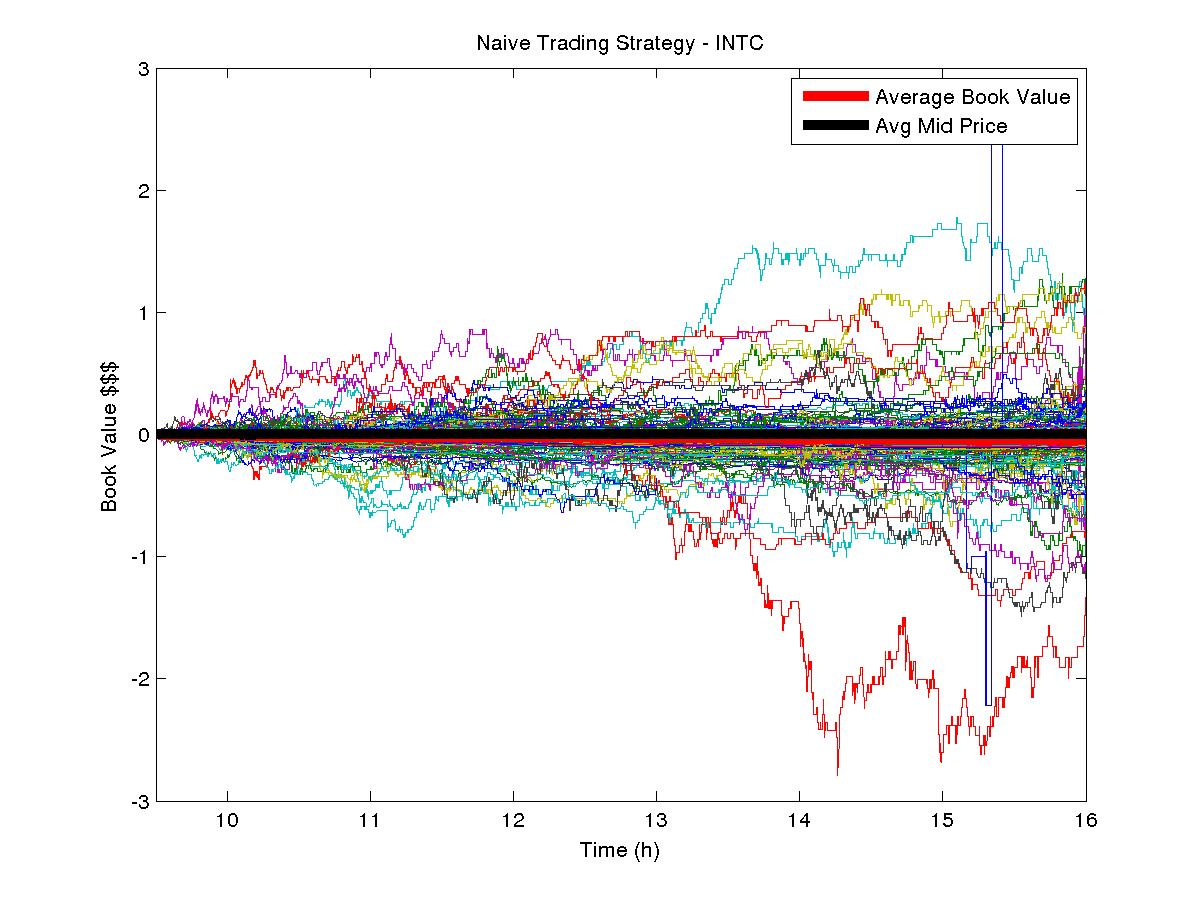
\includegraphics[width=\textwidth]{fig-INTC-year-bookvals}
  \caption{INTC: Bookvalue against time of trading day.}
\end{figure}

\begin{figure}
  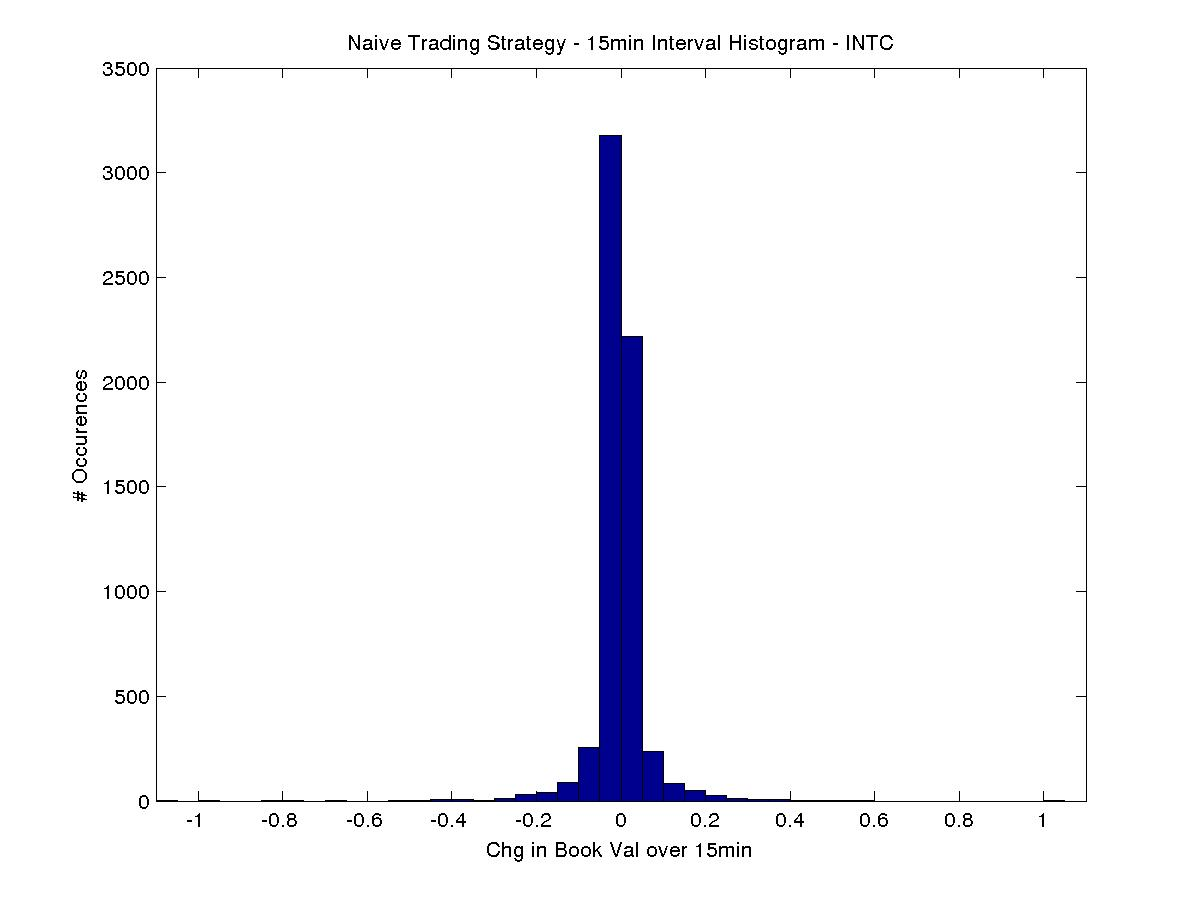
\includegraphics[width=\textwidth]{fig-INTC-15min-hist} \\
  \caption{INTC: Histogram of 15min bookvalue changes.}
\end{figure}

\begin{figure}[h]
  \centering
  \begin{tabular}{cc}
  	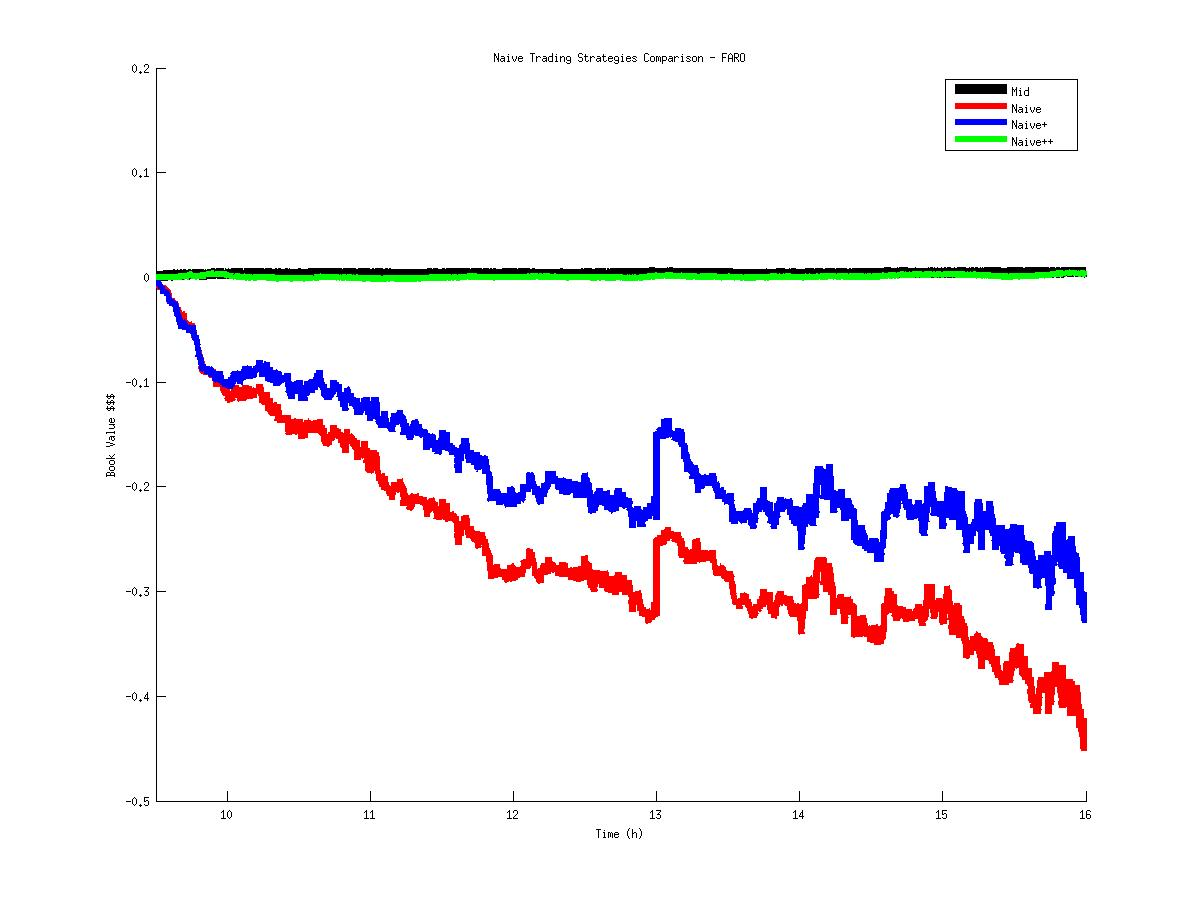
\includegraphics[width=0.45\textwidth]{fig-strategycompare-fixed-FARO} & 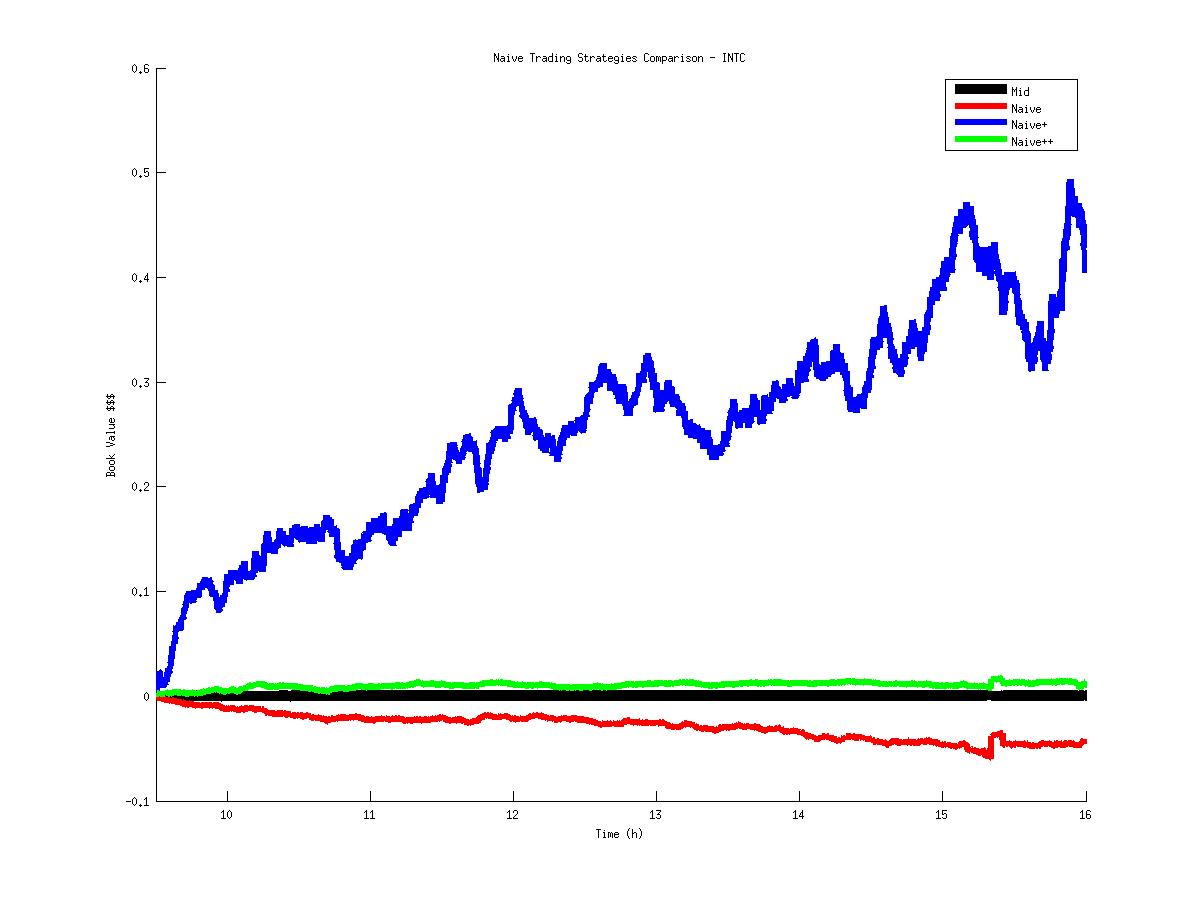
\includegraphics[width=0.45\textwidth]{fig-strategycompare-fixed-INTC} \\
  	FARO & INTC \\
  	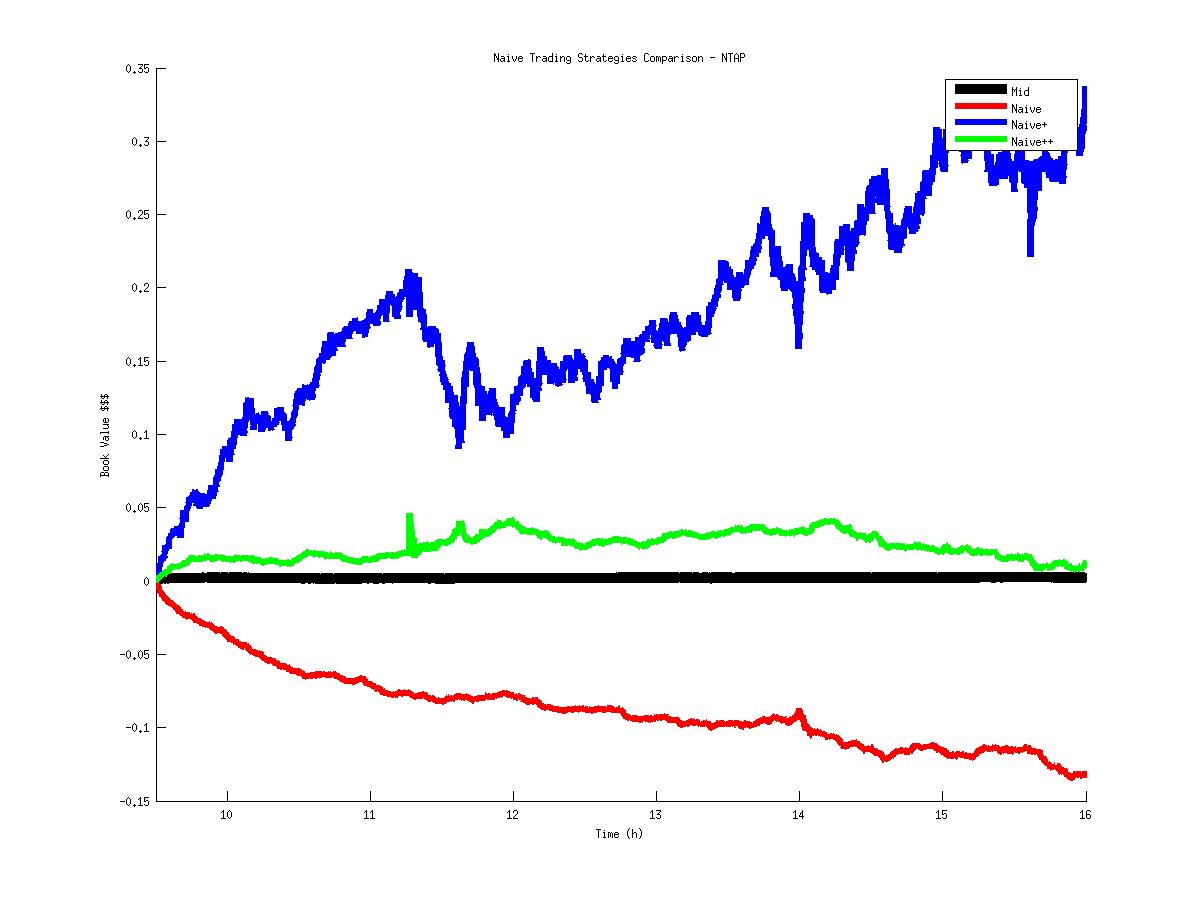
\includegraphics[width=0.45\textwidth]{fig-strategycompare-fixed-NTAP} & 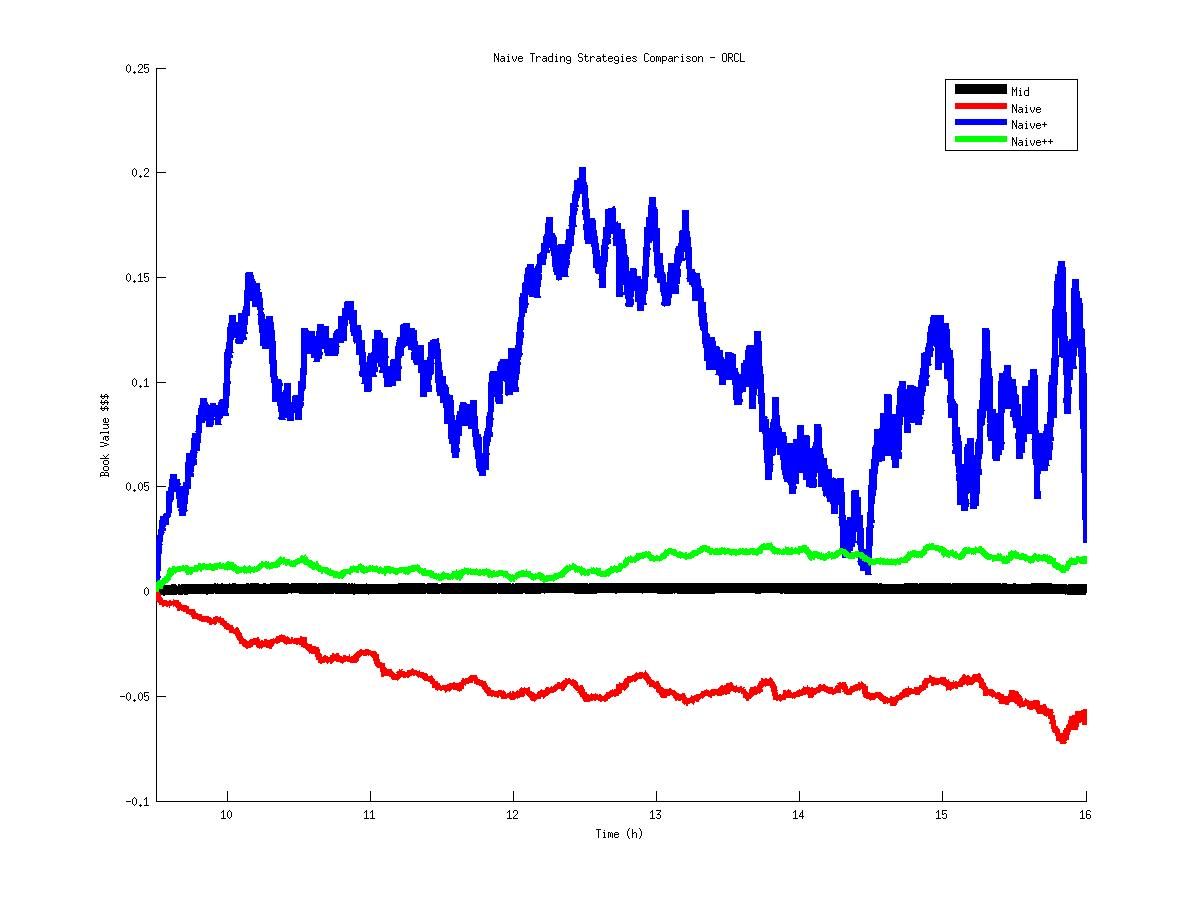
\includegraphics[width=0.45\textwidth]{fig-strategycompare-fixed-ORCL} \\
  	  	NTAP & ORCL \\
    \multicolumn{2}{c}{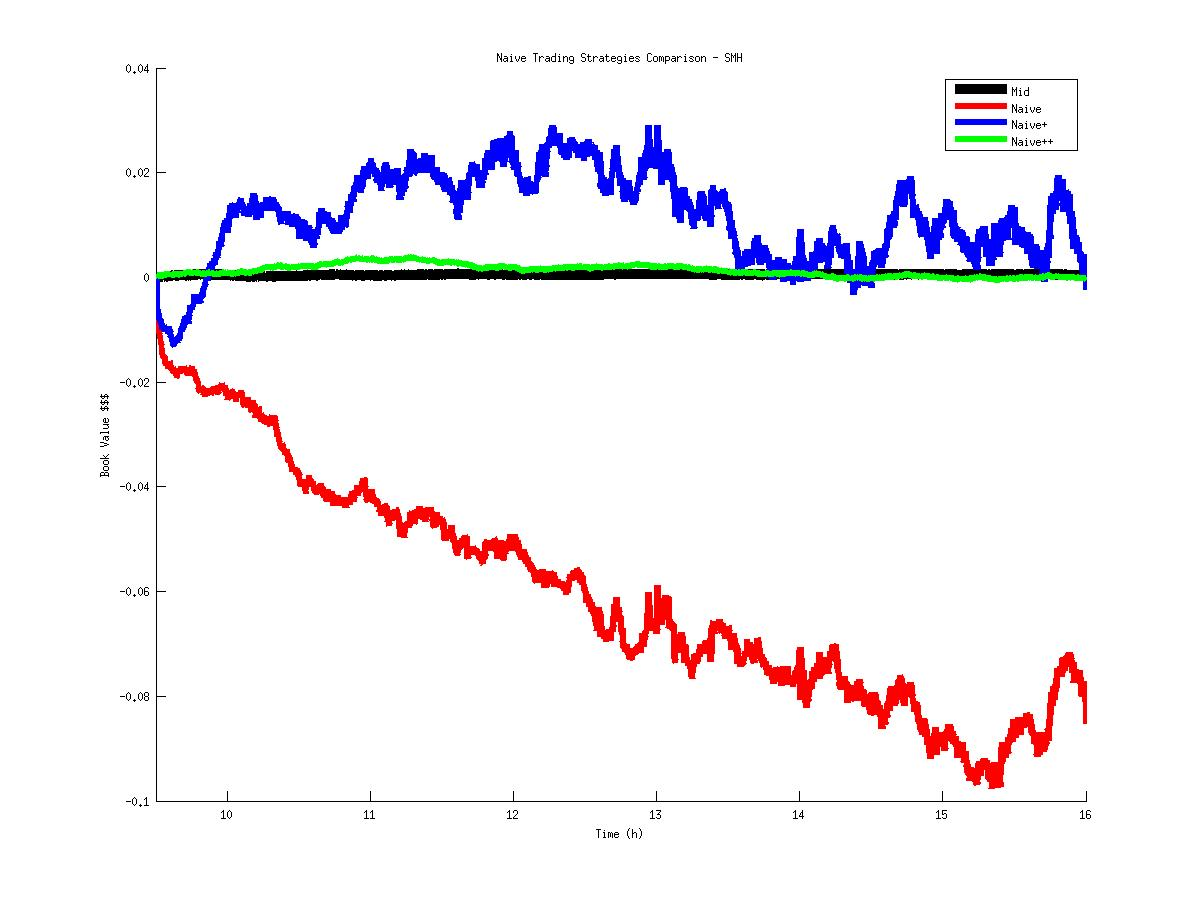
\includegraphics[width=0.45\textwidth]{fig-strategycompare-fixed-SMH} }\\
    \multicolumn{2}{c}{SMH}  	
  \end{tabular}
  \caption{Comparison of Naive (red), Naive+ (blue), and Naive++ (green) trading strategies, with benchmark Midprice (black). Plotted are bookvalues against time of trading day, averaged across trading year.}
  \label{fig:comp}
\end{figure}

\section*{Conclusions from Naive Trading Strategies}

To properly compare the Naive trading strategies, it must be understood that the Naive+ strategy has the Naive built into it - thus it's actually the difference between the two that needs to be assessed to ascertain the effect of posting Limit Orders when no price change is predicted. As seen in Figure \ref{fig:comp}, the Naive trading strategy on average underperformed the average mid price, while the Naive+ (adding at-the-touch limit orders when no change was predicted) and Naive++ (adding limit orders to adversely selecting agents that traded against the price change momentum) strategies both on average generated revenue. 

\paragraph{Question 1} Why is the Naive strategy producing, on average, normalized losses? Especially so when considering that we are \underline{in-sample backtesting}. On calibration, we see that our intra-day sharpe ratio is around 0.01 or 0.02 when we choose our optimal parameters, so at the very least on the calibration date the strategy produces positive returns. The remainder of the calendar days are out-of-sample, as the parameters are (likely) not optimal. This suggests non-stationary data, and in particular not every day can be modelled by the same Markov chain. The problem may be exaggerated by the fact that we're calibrating on the first trading day of the calendar year, when we might expect reduced, or at least non-representative, trading activity. Further, we're currently obtaining the $\mat{P_C}$ probability matrix using only bid-side data, not sell-side or mid, and we're ignoring the bid-ask spread. Thus predicting a ``price change'' may be insufficient when considering a monetizable opportunity, as we won't be able to profit off a predicted increase followed by a predicted decrease unless the interim mid-price move is greater than the bid-ask spread (assuming constant spread). This suggests a potential straightforward modification to the strategy.

\paragraph{Question 2} Why do the Naive+ and ++ strategies outperform the Naive strategy? This is particularly interesting since the probabilities are being obtained from the same matrix. The obvious difference between the successful and nonsuccessful strategies is that the former (a) uses limit orders, and (b) executes when we predict a zero change, whereas the latter uses (a) market orders, and (b) executes when we do predict nonzero change.

(a) obviously leads to a different transaction price being used: if I buy with a LO I'm paying the bid price, whereas buying with a MO I pay the ask price. If I value the stock using the mid price, and the mid price doesn't move as a result of my transaction, then with LO I'm buying the asset for less than I'm valuing it at, and with MO I'm paying more than its value.

(b) seems to be the largest flaw in the Naive strategy, to which there are two factors. One, we are not predicting the magnitude of the price change, only whether it is zero or nonzero. Two, from the probabilities presented above, \textit{we will only predict a price change if we've already seen a price change}. Thus we're effectively reacting too late. 

Here's how this works adversely. Suppose a stock has bid/ask quotes of \$9.99/\$10.01, for a bid-ask spread of \$0.02 and a mid of \$10.

\begin{enumerate}
\item Imbalance = 1 (pressure for upward price move). [$NPV = 0$]
\item Bid/ask goes up to \$10.00/\$10.02. [$NPV = 0$]
\item Imbalance = 1. We predict another $>0$ price change. [$NPV = 0$]
\item We buy 1 share (at \$10.02). [$NPV = -0.01$]
\item Bid/ask goes up to \$10.01/\$10.03. [$NPV = 0$]
\item Imbalance = -1 (pressure for a downward move). [$NPV = 0$]
\item Bid/ask goes down to \$10.00/\$10.02. [$NPV = -0.01$]
\item Imbalance = -1. We predict another $<0$ price change. 
\item We sell 1 share (at \$10.00). [$NPV = -0.02$]
\item Bid/ask goes down to \$9.99/\$10.01. [$NPV = -0.02$]
\end{enumerate}

In this example the price goes up and back down by two cents to return to where it started, and in the process we lost \$0.02. Now imagine what happens if we price goes up by one cent, up by one cent, then down by ten cents, down by one cent. In this case we lose \$0.11. We're unable to predict that initial upward or downward price change, and only react to it. 

\paragraph{Ideas to Explore and Next Steps}
\begin{itemize}
\item Model the mid price instead of the bid or ask, hold the bid-ask spread as a constant (average observed), and predict price changes at least as great as the spread, instead of simply non-zero.
\item Calculate imbalance using a weighted average of the best $n$ bid (resp. ask) prices. This may reduce noise in the signal, have an effect on the size of the imbalance averaging window, and be a stronger predictor.
\item Transition to exploring the stochastic control problem.
\end{itemize}

\end{document}
